% Generated by benchmarks/src/utils/make_table4_speedup_figures.py -- do not hand-edit.
\definecolor{sp0}{HTML}{2A78D6}
\definecolor{sp1}{HTML}{EB6834}
\definecolor{sp2}{HTML}{1BAF7A}
\pgfdeclareplotmark{heptagon*}{\pgfpathmoveto{\pgfqpointpolar{90.00}{\pgfplotmarksize}}\pgfpathlineto{\pgfqpointpolar{141.43}{\pgfplotmarksize}}\pgfpathlineto{\pgfqpointpolar{192.86}{\pgfplotmarksize}}\pgfpathlineto{\pgfqpointpolar{244.29}{\pgfplotmarksize}}\pgfpathlineto{\pgfqpointpolar{295.71}{\pgfplotmarksize}}\pgfpathlineto{\pgfqpointpolar{347.14}{\pgfplotmarksize}}\pgfpathlineto{\pgfqpointpolar{38.57}{\pgfplotmarksize}}\pgfpathclose\pgfusepathqfill}
\pgfdeclareplotmark{octagon*}{\pgfpathmoveto{\pgfqpointpolar{90.00}{\pgfplotmarksize}}\pgfpathlineto{\pgfqpointpolar{135.00}{\pgfplotmarksize}}\pgfpathlineto{\pgfqpointpolar{180.00}{\pgfplotmarksize}}\pgfpathlineto{\pgfqpointpolar{225.00}{\pgfplotmarksize}}\pgfpathlineto{\pgfqpointpolar{270.00}{\pgfplotmarksize}}\pgfpathlineto{\pgfqpointpolar{315.00}{\pgfplotmarksize}}\pgfpathlineto{\pgfqpointpolar{0.00}{\pgfplotmarksize}}\pgfpathlineto{\pgfqpointpolar{45.00}{\pgfplotmarksize}}\pgfpathclose\pgfusepathqfill}
\begin{figure*}[!t]
    \centering
    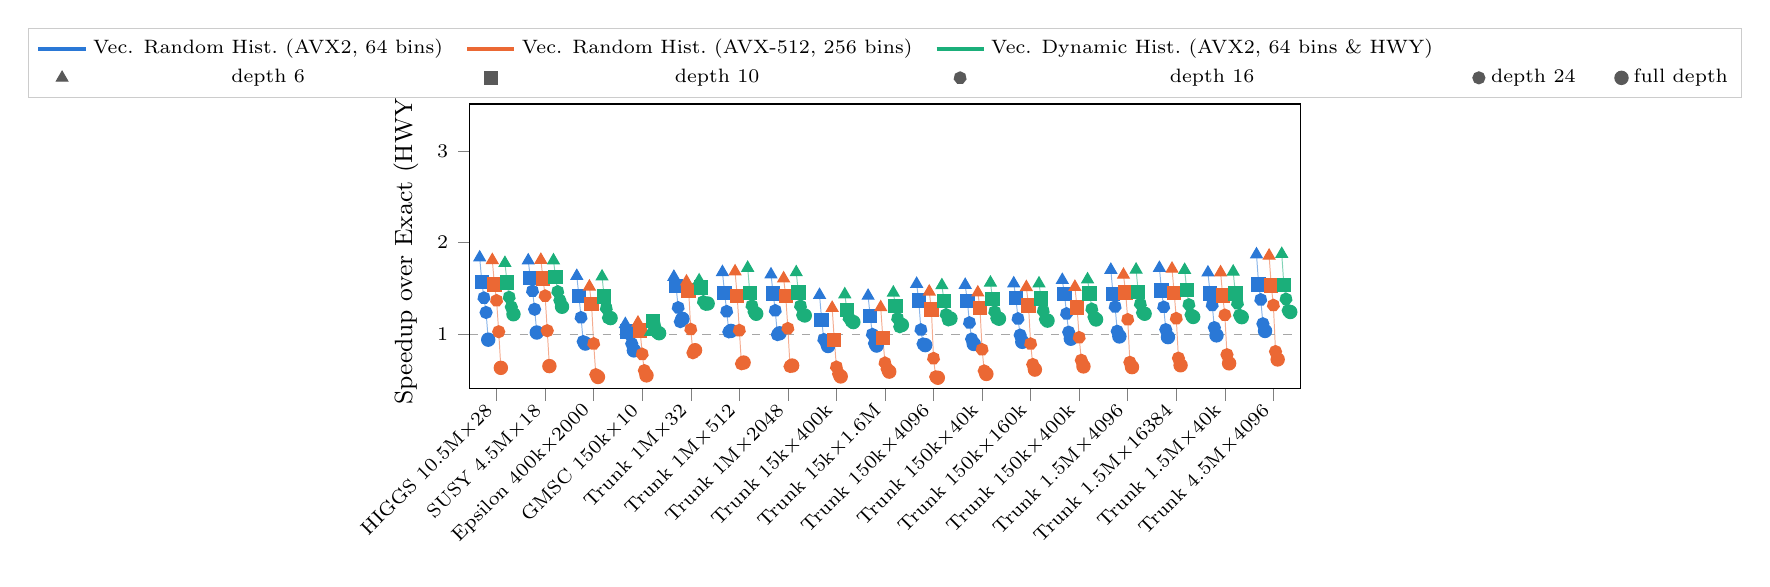
\begin{tikzpicture}
    \begin{axis}[
        width=\textwidth, height=5.2cm,
        xmin=0.45, xmax=17.55,
        ymin=0.41, ymax=3.51,
        xtick={1,2,3,4,5,6,7,8,9,10,11,12,13,14,15,16,17},
        xticklabels={HIGGS 10.5M$\times$28, SUSY 4.5M$\times$18, Epsilon 400k$\times$2000, GMSC 150k$\times$10, Trunk 1M$\times$32, Trunk 1M$\times$512, Trunk 1M$\times$2048, Trunk 15k$\times$400k, Trunk 15k$\times$1.6M, Trunk 150k$\times$4096, Trunk 150k$\times$40k, Trunk 150k$\times$160k, Trunk 150k$\times$400k, Trunk 1.5M$\times$4096, Trunk 1.5M$\times$16384, Trunk 1.5M$\times$40k, Trunk 4.5M$\times$4096},
        xticklabel style={rotate=45, anchor=east, font=\scriptsize},
        yticklabel style={font=\scriptsize},
        ylabel={Speedup over Exact (HWY)},
        ylabel style={font=\small},
        tick align=outside, tick pos=left,
        legend columns=5, legend style={font=\scriptsize, draw=gray!40,
            at={(0.5,1.02)}, anchor=south, /tikz/every even column/.append style={column sep=6pt}},
    ]
    \addplot[color=sp0, line width=0.35pt, opacity=0.55, mark=none, forget plot] coordinates {(0.652,1.8390) (0.696,1.5752) (0.740,1.4010) (0.784,1.2413) (0.828,0.9455)};
    \addplot[color=sp0, line width=0.35pt, opacity=0.55, mark=none, forget plot] coordinates {(1.652,1.8067) (1.696,1.6161) (1.740,1.4750) (1.784,1.2760) (1.828,1.0233)};
    \addplot[color=sp0, line width=0.35pt, opacity=0.55, mark=none, forget plot] coordinates {(2.652,1.6381) (2.696,1.4221) (2.740,1.1872) (2.784,0.9249) (2.828,0.9033)};
    \addplot[color=sp0, line width=0.35pt, opacity=0.55, mark=none, forget plot] coordinates {(3.652,1.1144) (3.696,1.0343) (3.740,1.0043) (3.784,0.9016) (3.828,0.8288)};
    \addplot[color=sp0, line width=0.35pt, opacity=0.55, mark=none, forget plot] coordinates {(4.652,1.6285) (4.696,1.5296) (4.740,1.2953) (4.784,1.1411) (4.828,1.1717)};
    \addplot[color=sp0, line width=0.35pt, opacity=0.55, mark=none, forget plot] coordinates {(5.652,1.6800) (5.696,1.4553) (5.740,1.2538) (5.784,1.0300) (5.828,1.0409)};
    \addplot[color=sp0, line width=0.35pt, opacity=0.55, mark=none, forget plot] coordinates {(6.652,1.6545) (6.696,1.4458) (6.740,1.2629) (6.784,1.0000) (6.828,1.0148)};
    \addplot[color=sp0, line width=0.35pt, opacity=0.55, mark=none, forget plot] coordinates {(7.652,1.4313) (7.696,1.1607) (7.740,0.9479) (7.784,0.9125) (7.828,0.8764)};
    \addplot[color=sp0, line width=0.35pt, opacity=0.55, mark=none, forget plot] coordinates {(8.652,1.4222) (8.696,1.2007) (8.740,1.0044) (8.784,0.9056) (8.828,0.8815)};
    \addplot[color=sp0, line width=0.35pt, opacity=0.55, mark=none, forget plot] coordinates {(9.652,1.5522) (9.696,1.3696) (9.740,1.0544) (9.784,0.8992) (9.828,0.8861)};
    \addplot[color=sp0, line width=0.35pt, opacity=0.55, mark=none, forget plot] coordinates {(10.652,1.5408) (10.696,1.3643) (10.740,1.1306) (10.784,0.9518) (10.828,0.8989)};
    \addplot[color=sp0, line width=0.35pt, opacity=0.55, mark=none, forget plot] coordinates {(11.652,1.5567) (11.696,1.3981) (11.740,1.1743) (11.784,0.9952) (11.828,0.9219)};
    \addplot[color=sp0, line width=0.35pt, opacity=0.55, mark=none, forget plot] coordinates {(12.652,1.5946) (12.696,1.4421) (12.740,1.2289) (12.784,1.0273) (12.828,0.9558)};
    \addplot[color=sp0, line width=0.35pt, opacity=0.55, mark=none, forget plot] coordinates {(13.652,1.7047) (13.696,1.4454) (13.740,1.3043) (13.784,1.0370) (13.828,0.9804)};
    \addplot[color=sp0, line width=0.35pt, opacity=0.55, mark=none, forget plot] coordinates {(14.652,1.7253) (14.696,1.4792) (14.740,1.3010) (14.784,1.0549) (14.828,0.9732)};
    \addplot[color=sp0, line width=0.35pt, opacity=0.55, mark=none, forget plot] coordinates {(15.652,1.6752) (15.696,1.4486) (15.740,1.3221) (15.784,1.0768) (15.828,0.9923)};
    \addplot[color=sp0, line width=0.35pt, opacity=0.55, mark=none, forget plot] coordinates {(16.652,1.8725) (16.696,1.5460) (16.740,1.3818) (16.784,1.1188) (16.828,1.0402)};
    \addplot[color=sp0, mark=triangle*, mark size=2.4pt, only marks, forget plot] coordinates {(0.652,1.8390) (1.652,1.8067) (2.652,1.6381) (3.652,1.1144) (4.652,1.6285) (5.652,1.6800) (6.652,1.6545) (7.652,1.4313) (8.652,1.4222) (9.652,1.5522) (10.652,1.5408) (11.652,1.5567) (12.652,1.5946) (13.652,1.7047) (14.652,1.7253) (15.652,1.6752) (16.652,1.8725)};
    \addplot[color=sp0, mark=square*, mark size=2.4pt, only marks, forget plot] coordinates {(0.696,1.5752) (1.696,1.6161) (2.696,1.4221) (3.696,1.0343) (4.696,1.5296) (5.696,1.4553) (6.696,1.4458) (7.696,1.1607) (8.696,1.2007) (9.696,1.3696) (10.696,1.3643) (11.696,1.3981) (12.696,1.4421) (13.696,1.4454) (14.696,1.4792) (15.696,1.4486) (16.696,1.5460)};
    \addplot[color=sp0, mark=heptagon*, mark size=2.4pt, only marks, forget plot] coordinates {(0.740,1.4010) (1.740,1.4750) (2.740,1.1872) (3.740,1.0043) (4.740,1.2953) (5.740,1.2538) (6.740,1.2629) (7.740,0.9479) (8.740,1.0044) (9.740,1.0544) (10.740,1.1306) (11.740,1.1743) (12.740,1.2289) (13.740,1.3043) (14.740,1.3010) (15.740,1.3221) (16.740,1.3818)};
    \addplot[color=sp0, mark=octagon*, mark size=2.4pt, only marks, forget plot] coordinates {(0.784,1.2413) (1.784,1.2760) (2.784,0.9249) (3.784,0.9016) (4.784,1.1411) (5.784,1.0300) (6.784,1.0000) (7.784,0.9125) (8.784,0.9056) (9.784,0.8992) (10.784,0.9518) (11.784,0.9952) (12.784,1.0273) (13.784,1.0370) (14.784,1.0549) (15.784,1.0768) (16.784,1.1188)};
    \addplot[color=sp0, mark=*, mark size=2.4pt, only marks, forget plot] coordinates {(0.828,0.9455) (1.828,1.0233) (2.828,0.9033) (3.828,0.8288) (4.828,1.1717) (5.828,1.0409) (6.828,1.0148) (7.828,0.8764) (8.828,0.8815) (9.828,0.8861) (10.828,0.8989) (11.828,0.9219) (12.828,0.9558) (13.828,0.9804) (14.828,0.9732) (15.828,0.9923) (16.828,1.0402)};
    \addplot[color=sp1, line width=0.35pt, opacity=0.55, mark=none, forget plot] coordinates {(0.912,1.8106) (0.956,1.5450) (1.000,1.3717) (1.044,1.0319) (1.088,0.6390)};
    \addplot[color=sp1, line width=0.35pt, opacity=0.55, mark=none, forget plot] coordinates {(1.912,1.8132) (1.956,1.6103) (2.000,1.4224) (2.044,1.0429) (2.088,0.6579)};
    \addplot[color=sp1, line width=0.35pt, opacity=0.55, mark=none, forget plot] coordinates {(2.912,1.5225) (2.956,1.3344) (3.000,0.9026) (3.044,0.5651) (3.088,0.5397)};
    \addplot[color=sp1, line width=0.35pt, opacity=0.55, mark=none, forget plot] coordinates {(3.912,1.1297) (3.956,1.0446) (4.000,0.7884) (4.044,0.6091) (4.088,0.5568)};
    \addplot[color=sp1, line width=0.35pt, opacity=0.55, mark=none, forget plot] coordinates {(4.912,1.5772) (4.956,1.4814) (5.000,1.0588) (5.044,0.8023) (5.088,0.8309)};
    \addplot[color=sp1, line width=0.35pt, opacity=0.55, mark=none, forget plot] coordinates {(5.912,1.6874) (5.956,1.4182) (6.000,1.0478) (6.044,0.6830) (6.088,0.6964)};
    \addplot[color=sp1, line width=0.35pt, opacity=0.55, mark=none, forget plot] coordinates {(6.912,1.6115) (6.956,1.4181) (7.000,1.0681) (7.044,0.6539) (7.088,0.6638)};
    \addplot[color=sp1, line width=0.35pt, opacity=0.55, mark=none, forget plot] coordinates {(7.912,1.2908) (7.956,0.9412) (8.000,0.6491) (8.044,0.5728) (8.088,0.5454)};
    \addplot[color=sp1, line width=0.35pt, opacity=0.55, mark=none, forget plot] coordinates {(8.912,1.2972) (8.956,0.9611) (9.000,0.6930) (9.044,0.6264) (9.088,0.5977)};
    \addplot[color=sp1, line width=0.35pt, opacity=0.55, mark=none, forget plot] coordinates {(9.912,1.4678) (9.956,1.2718) (10.000,0.7430) (10.044,0.5409) (10.088,0.5311)};
    \addplot[color=sp1, line width=0.35pt, opacity=0.55, mark=none, forget plot] coordinates {(10.912,1.4577) (10.956,1.2893) (11.000,0.8387) (11.044,0.6058) (11.088,0.5726)};
    \addplot[color=sp1, line width=0.35pt, opacity=0.55, mark=none, forget plot] coordinates {(11.912,1.5162) (11.956,1.3156) (12.000,0.9010) (12.044,0.6756) (12.088,0.6199)};
    \addplot[color=sp1, line width=0.35pt, opacity=0.55, mark=none, forget plot] coordinates {(12.912,1.5191) (12.956,1.2947) (13.000,0.9700) (13.044,0.7210) (13.088,0.6546)};
    \addplot[color=sp1, line width=0.35pt, opacity=0.55, mark=none, forget plot] coordinates {(13.912,1.6511) (13.956,1.4596) (14.000,1.1652) (14.044,0.6986) (14.088,0.6469)};
    \addplot[color=sp1, line width=0.35pt, opacity=0.55, mark=none, forget plot] coordinates {(14.912,1.7167) (14.956,1.4548) (15.000,1.1771) (15.044,0.7445) (15.088,0.6670)};
    \addplot[color=sp1, line width=0.35pt, opacity=0.55, mark=none, forget plot] coordinates {(15.912,1.6774) (15.956,1.4252) (16.000,1.2141) (16.044,0.7822) (16.088,0.6880)};
    \addplot[color=sp1, line width=0.35pt, opacity=0.55, mark=none, forget plot] coordinates {(16.912,1.8590) (16.956,1.5332) (17.000,1.3205) (17.044,0.8161) (17.088,0.7302)};
    \addplot[color=sp1, mark=triangle*, mark size=2.4pt, only marks, forget plot] coordinates {(0.912,1.8106) (1.912,1.8132) (2.912,1.5225) (3.912,1.1297) (4.912,1.5772) (5.912,1.6874) (6.912,1.6115) (7.912,1.2908) (8.912,1.2972) (9.912,1.4678) (10.912,1.4577) (11.912,1.5162) (12.912,1.5191) (13.912,1.6511) (14.912,1.7167) (15.912,1.6774) (16.912,1.8590)};
    \addplot[color=sp1, mark=square*, mark size=2.4pt, only marks, forget plot] coordinates {(0.956,1.5450) (1.956,1.6103) (2.956,1.3344) (3.956,1.0446) (4.956,1.4814) (5.956,1.4182) (6.956,1.4181) (7.956,0.9412) (8.956,0.9611) (9.956,1.2718) (10.956,1.2893) (11.956,1.3156) (12.956,1.2947) (13.956,1.4596) (14.956,1.4548) (15.956,1.4252) (16.956,1.5332)};
    \addplot[color=sp1, mark=heptagon*, mark size=2.4pt, only marks, forget plot] coordinates {(1.000,1.3717) (2.000,1.4224) (3.000,0.9026) (4.000,0.7884) (5.000,1.0588) (6.000,1.0478) (7.000,1.0681) (8.000,0.6491) (9.000,0.6930) (10.000,0.7430) (11.000,0.8387) (12.000,0.9010) (13.000,0.9700) (14.000,1.1652) (15.000,1.1771) (16.000,1.2141) (17.000,1.3205)};
    \addplot[color=sp1, mark=octagon*, mark size=2.4pt, only marks, forget plot] coordinates {(1.044,1.0319) (2.044,1.0429) (3.044,0.5651) (4.044,0.6091) (5.044,0.8023) (6.044,0.6830) (7.044,0.6539) (8.044,0.5728) (9.044,0.6264) (10.044,0.5409) (11.044,0.6058) (12.044,0.6756) (13.044,0.7210) (14.044,0.6986) (15.044,0.7445) (16.044,0.7822) (17.044,0.8161)};
    \addplot[color=sp1, mark=*, mark size=2.4pt, only marks, forget plot] coordinates {(1.088,0.6390) (2.088,0.6579) (3.088,0.5397) (4.088,0.5568) (5.088,0.8309) (6.088,0.6964) (7.088,0.6638) (8.088,0.5454) (9.088,0.5977) (10.088,0.5311) (11.088,0.5726) (12.088,0.6199) (13.088,0.6546) (14.088,0.6469) (15.088,0.6670) (16.088,0.6880) (17.088,0.7302)};
    \addplot[color=sp2, line width=0.35pt, opacity=0.55, mark=none, forget plot] coordinates {(1.172,1.7791) (1.216,1.5687) (1.260,1.4075) (1.304,1.3012) (1.348,1.2221)};
    \addplot[color=sp2, line width=0.35pt, opacity=0.55, mark=none, forget plot] coordinates {(2.172,1.8073) (2.216,1.6256) (2.260,1.4686) (2.304,1.3732) (2.348,1.3035)};
    \addplot[color=sp2, line width=0.35pt, opacity=0.55, mark=none, forget plot] coordinates {(3.172,1.6316) (3.216,1.4136) (3.260,1.2871) (3.304,1.1827) (3.348,1.1802)};
    \addplot[color=sp2, line width=0.35pt, opacity=0.55, mark=none, forget plot] coordinates {(4.172,1.0287) (4.216,1.1491) (4.260,1.0982) (4.304,1.0249) (4.348,1.0152)};
    \addplot[color=sp2, line width=0.35pt, opacity=0.55, mark=none, forget plot] coordinates {(5.172,1.5895) (5.216,1.5138) (5.260,1.3596) (5.304,1.3301) (5.348,1.3387)};
    \addplot[color=sp2, line width=0.35pt, opacity=0.55, mark=none, forget plot] coordinates {(6.172,1.7266) (6.216,1.4554) (6.260,1.3148) (6.304,1.2471) (6.348,1.2274)};
    \addplot[color=sp2, line width=0.35pt, opacity=0.55, mark=none, forget plot] coordinates {(7.172,1.6781) (7.216,1.4583) (7.260,1.3126) (7.304,1.2125) (7.348,1.2089)};
    \addplot[color=sp2, line width=0.35pt, opacity=0.55, mark=none, forget plot] coordinates {(8.172,1.4379) (8.216,1.2706) (8.260,1.1784) (8.304,1.1460) (8.348,1.1366)};
    \addplot[color=sp2, line width=0.35pt, opacity=0.55, mark=none, forget plot] coordinates {(9.172,1.4571) (9.216,1.3149) (9.260,1.1762) (9.304,1.0858) (9.348,1.1058)};
    \addplot[color=sp2, line width=0.35pt, opacity=0.55, mark=none, forget plot] coordinates {(10.172,1.5367) (10.216,1.3665) (10.260,1.2190) (10.304,1.1604) (10.348,1.1756)};
    \addplot[color=sp2, line width=0.35pt, opacity=0.55, mark=none, forget plot] coordinates {(11.172,1.5655) (11.216,1.3848) (11.260,1.2495) (11.304,1.1775) (11.348,1.1733)};
    \addplot[color=sp2, line width=0.35pt, opacity=0.55, mark=none, forget plot] coordinates {(12.172,1.5563) (12.216,1.3945) (12.260,1.2583) (12.304,1.1680) (12.348,1.1529)};
    \addplot[color=sp2, line width=0.35pt, opacity=0.55, mark=none, forget plot] coordinates {(13.172,1.6007) (13.216,1.4485) (13.260,1.2794) (13.304,1.1919) (13.348,1.1651)};
    \addplot[color=sp2, line width=0.35pt, opacity=0.55, mark=none, forget plot] coordinates {(14.172,1.7066) (14.216,1.4638) (14.260,1.3329) (14.304,1.2379) (14.348,1.2275)};
    \addplot[color=sp2, line width=0.35pt, opacity=0.55, mark=none, forget plot] coordinates {(15.172,1.7034) (15.216,1.4828) (15.260,1.3268) (15.304,1.2156) (15.348,1.1926)};
    \addplot[color=sp2, line width=0.35pt, opacity=0.55, mark=none, forget plot] coordinates {(16.172,1.6852) (16.216,1.4468) (16.260,1.3398) (16.304,1.2115) (16.348,1.1901)};
    \addplot[color=sp2, line width=0.35pt, opacity=0.55, mark=none, forget plot] coordinates {(17.172,1.8774) (17.216,1.5400) (17.260,1.3879) (17.304,1.2622) (17.348,1.2465)};
    \addplot[color=sp2, mark=triangle*, mark size=2.4pt, only marks, forget plot] coordinates {(1.172,1.7791) (2.172,1.8073) (3.172,1.6316) (4.172,1.0287) (5.172,1.5895) (6.172,1.7266) (7.172,1.6781) (8.172,1.4379) (9.172,1.4571) (10.172,1.5367) (11.172,1.5655) (12.172,1.5563) (13.172,1.6007) (14.172,1.7066) (15.172,1.7034) (16.172,1.6852) (17.172,1.8774)};
    \addplot[color=sp2, mark=square*, mark size=2.4pt, only marks, forget plot] coordinates {(1.216,1.5687) (2.216,1.6256) (3.216,1.4136) (4.216,1.1491) (5.216,1.5138) (6.216,1.4554) (7.216,1.4583) (8.216,1.2706) (9.216,1.3149) (10.216,1.3665) (11.216,1.3848) (12.216,1.3945) (13.216,1.4485) (14.216,1.4638) (15.216,1.4828) (16.216,1.4468) (17.216,1.5400)};
    \addplot[color=sp2, mark=heptagon*, mark size=2.4pt, only marks, forget plot] coordinates {(1.260,1.4075) (2.260,1.4686) (3.260,1.2871) (4.260,1.0982) (5.260,1.3596) (6.260,1.3148) (7.260,1.3126) (8.260,1.1784) (9.260,1.1762) (10.260,1.2190) (11.260,1.2495) (12.260,1.2583) (13.260,1.2794) (14.260,1.3329) (15.260,1.3268) (16.260,1.3398) (17.260,1.3879)};
    \addplot[color=sp2, mark=octagon*, mark size=2.4pt, only marks, forget plot] coordinates {(1.304,1.3012) (2.304,1.3732) (3.304,1.1827) (4.304,1.0249) (5.304,1.3301) (6.304,1.2471) (7.304,1.2125) (8.304,1.1460) (9.304,1.0858) (10.304,1.1604) (11.304,1.1775) (12.304,1.1680) (13.304,1.1919) (14.304,1.2379) (15.304,1.2156) (16.304,1.2115) (17.304,1.2622)};
    \addplot[color=sp2, mark=*, mark size=2.4pt, only marks, forget plot] coordinates {(1.348,1.2221) (2.348,1.3035) (3.348,1.1802) (4.348,1.0152) (5.348,1.3387) (6.348,1.2274) (7.348,1.2089) (8.348,1.1366) (9.348,1.1058) (10.348,1.1756) (11.348,1.1733) (12.348,1.1529) (13.348,1.1651) (14.348,1.2275) (15.348,1.1926) (16.348,1.1901) (17.348,1.2465)};
    \addplot[color=sp0, mark=none, line width=1.4pt] coordinates {(-9,1) (-8,1)};
    \addlegendentry{Vec. Random Hist.\ (AVX2, 64 bins)}
    \addplot[color=sp1, mark=none, line width=1.4pt] coordinates {(-9,1) (-8,1)};
    \addlegendentry{Vec. Random Hist.\ (AVX-512, 256 bins)}
    \addplot[color=sp2, mark=none, line width=1.4pt] coordinates {(-9,1) (-8,1)};
    \addlegendentry{Vec. Dynamic Hist.\ (AVX2, 64 bins \& HWY)}
    \addlegendimage{empty legend}
    \addlegendentry{}
    \addlegendimage{empty legend}
    \addlegendentry{}
    \addplot[color=black!65, mark=triangle*, mark size=2.4pt, only marks] coordinates {(-9,1)};
    \addlegendentry{depth 6}
    \addplot[color=black!65, mark=square*, mark size=2.4pt, only marks] coordinates {(-9,1)};
    \addlegendentry{depth 10}
    \addplot[color=black!65, mark=heptagon*, mark size=2.4pt, only marks] coordinates {(-9,1)};
    \addlegendentry{depth 16}
    \addplot[color=black!65, mark=octagon*, mark size=2.4pt, only marks] coordinates {(-9,1)};
    \addlegendentry{depth 24}
    \addplot[color=black!65, mark=*, mark size=2.4pt, only marks] coordinates {(-9,1)};
    \addlegendentry{full depth}
    \draw[gray!70, dashed, line width=0.6pt] (axis cs:0.45,1) -- (axis cs:17.55,1);
    \end{axis}
    \end{tikzpicture}
    \caption{Speedup over exact splitting (Highway VQSort) per dataset and tree depth, the cells of Table~\ref{tab:train-time-by-depth}; marks left to right = depths 6, 10, 16, 24, purity; dashed line = parity; single run.}
    \label{fig:speedup-by-depth-vs-exact}
\end{figure*}
